\documentclass[10pt,twocolumn,letterpaper]{article}

\usepackage{cvpr}
\usepackage{times}
\usepackage{epsfig}
\usepackage{graphicx}
\usepackage{amsmath}
\usepackage{amssymb}
%\usepackage{algorithmic}
\usepackage{algpseudocode}
\usepackage{enumitem}
\usepackage{listings}
\usepackage{amsmath}
\usepackage{algorithm,algpseudocode}
\lstset { %
    language=C++,
    %backgroundcolor=\color{gray!5}, % set backgroundcolor
    basicstyle=\footnotesize,% basic font setting
}



\usepackage{url}

% Include other packages here, before hyperref.

% If you comment hyperref and then uncomment it, you should delete
% egpaper.aux before re-running latex.  (Or just hit 'q' on the first latex
% run, let it finish, and you should be clear).
%\usepackage[pagebackref=true,breaklinks=true,letterpaper=true,colorlinks,bookmarks=false]{hyperref}

\cvprfinalcopy % *** Uncomment this line for the final submission

\def\cvprPaperID{****} % *** Enter the CVPR Paper ID here
\def\httilde{\mbox{\tt\raisebox{-.5ex}{\symbol{126}}}}

% Pages are numbered in submission mode, and unnumbered in camera-ready
\ifcvprfinal\pagestyle{empty}\fi


\newcommand\NoDo{\renewcommand\algorithmicdo{}}
\newcommand\ReDo{\renewcommand\algorithmicdo{\textbf{do}}}
\newcommand\NoThen{\renewcommand\algorithmicthen{}}
\newcommand\ReThen{\renewcommand\algorithmicthen{\textbf{then}}}

\begin{document}

%%%%%%%%% TITLE
\title{Bigrams/trigrams generation}

\author{Antonio Castellucci\\
{\tt\small antonio.castellucci@stud.unifi.it}
% For a paper whose authors are all at the same institution,
% omit the following lines up until the closing ``}''.
% Additional authors and addresses can be added with ``\and'',
% just like the second author.
% To save space, use either the email address or home page, not both
\and
Michela Crulli\\
{\tt\small michela.crulli@stud.unifi.it}
}

\maketitle
\thispagestyle{empty}

%%%%%%%%% ABSTRACT

\begin{abstract}
In this report, we describe a program which generates bigrams and trigrams with three different approaches: sequential, parallel and distributed.\\ 
Firstly we describe the technologies we use for each version and the logic we implement.\\
After, we compare average runtimes of the executions of different versions, commenting on the various test results and showing our opinion on the use case submitted.

\end{abstract}

%%%%%%%%% BODY TEXT
\section{Introduction}
An n-gram is a contiguous sequence of n items from a given text or speech.
The items can be letters, words but also syllables or phonemes.\\
N-grams can be very useful because, for example, if we assign a probability to the occurrence of an n-gram or to a word occurring next in a sequence of words, we can decide which n-grams can be chuncked together to form single entities (like "San Francisco"). It can also help make new word predictions and it can also help to make spelling error corrections. In our project we have decided to do letter's ngram.\\
In the first section we better define input/output for all implementations and introduce the technologies we use for the distributed implementation.
In the second section we describe datasets for testing and in third section the logic implemented in different approaches and then we show our test and results.

\vspace{5cm}
%-------------------------------------------------------------------------
\subsection{Input output structure}

For a more accurate comparison, we fix a priori the input and output structure for all implementations:\\ 
The program takes in input a folder with books (as txt files) and creates, like output, two text files, one with bigrams and the other one  with trigrams without mix up books's content.\\

\begin{figure}[H]
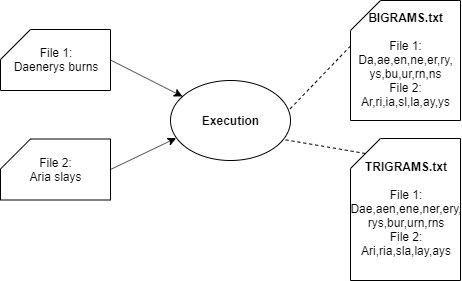
\includegraphics[width=\columnwidth]{template/latex/task.png}
\begin{center}
\caption{Scheme of input output structure.}
\label{fig:short}
\end{center}
\end{figure}
%------------------------------------------------------------------------
%-------------------------------------------------------------------------
\subsection{Hadoop}

Apache Hadoop is a collection of open-source software utilities that facilitate using a network of many computers to solve problems involving massive amounts of data and computation. It provides a software framework for distributed storage and processing of big data using the MapReduce programming model.\\
The core of Apache Hadoop consists of a storage part, known as Hadoop Distributed File System (HDFS), and a processing part which is a MapReduce programming model. Hadoop splits files into large blocks and distributes them across nodes in a cluster. It then transfers packaged code into nodes to process the data in parallel.\\
The Hadoop framework itself is mostly written in the Java programming language, with some native code in C and command line utilities written as shell scripts.\\
Though MapReduce Java code is common, any programming language can be used with Hadoop Streaming to implement the map and reduce parts of the user's program.\\\\
Hadoop is used for performing computations over large amounts of data.\\
Jobs might be bounded by the resources of IO (I/O intensive), CPU and Network. In the classic case of Hadoop usage it is performed local computations over huge amounts of input data while returning relatively small result set, which makes the task be more IO intensive than CPU and Network intensive, but it hugely depends on the job itself. Here are some examples:
\begin{itemize}
    \item IO Intensive job: read much data on the map side, but the result of map task is not that big.\\
    An example is calculating amount of rows in the input text, calculating the sum over some column from RCfile, getting the result of the Hive query over a single table with group by a column with relatively small cardinality. This would mean that the thing the job is doing is mostly reading data and make some simple processing over it.

    \item CPU Intensive job: when there is a need to perform some complex computations on the map or reduce side. For instance, you are doing some kind of the NLP (natural language processing) like tokenization, part of speech tagging, stemming and so on. Also if you store the data in a format with high compression rates data decompression might become the bottleneck of the process .
\end{itemize}
Our application is certainly i/o intensive but the size of output is approximately six times bigger than the input size, infact, we can easily verify that the output of our program for a input like:\\
“Lorem ipsum dolor sit amet” is:\\
“Lo,or,re,em,ip,ps,su,um,do,ol,lo,or,si,it,am,me,et” plus “Lor,ere,rem,ips,psu,sum,dol,olo,lor,sit,ame,met”\\
 
This consideration suggests that our case is not very appropriate to be implemented with Hadoop but we will see the tests what they tell us.

%-------------------------------------------------------------------------

\subsection{EMR (AWS)}

Amazon EMR is the industry-leading cloud-native big data platform, allowing teams to process vast amounts of data quickly, and cost-effectively at scale.\\
Using open-source tools such as Apache Spark, Apache Hive, Apache HBase, Apache Flink, and Apache Hadoop, coupled with the dynamic scalability of Amazon EC2 and scalable storage of Amazon S3 (which we use for storing input dataset and save our output for distributed implementation).\\
EMR gives analytical teams the engines and elasticity to run Petabyte-scale analysis for a fraction of the cost of traditional on-premise clusters. The S3 support enables S3-based data lakes to comply with data privacy laws, consume real time streams and change data capture logs, reinstate late arriving data, and track change history and rollback. 
By using the EMR File System (EMRFS) on an Amazon EMR cluster, you can leverage Amazon S3 as data layer for Hadoop. Amazon S3 is highly scalable, low cost, and designed for durability, making it a great data store for big data processing. By storing your data in Amazon S3, you can decouple your compute layer from your storage layer, allowing you to size your Amazon EMR cluster for the amount of CPU and memory required for your workloads instead of having extra nodes in your cluster to maximize on-cluster storage.\\

\begin{figure}[H]
\begin{center}
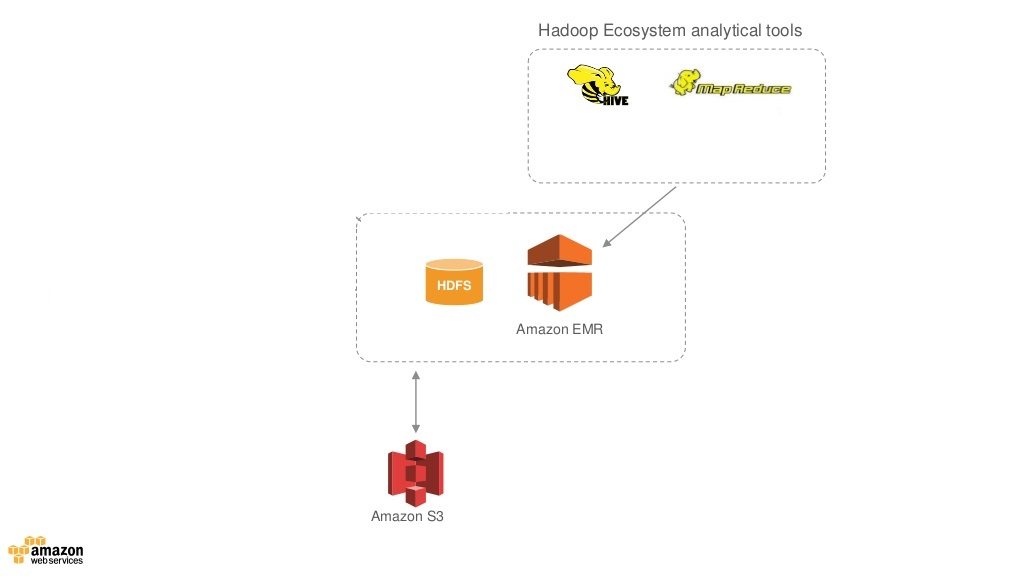
\includegraphics[width=\columnwidth]{template/latex/bigData.jpg}
\caption{Scheme of Hadoop application running on EMR cluster with S3 data support.}
\label{fig:short}
\end{center}
\end{figure}

\section{Dataset}
All project's test are executed on a collection of 3000 books acquired from Gutenberg's Project and on the collection's subsets:
\setlist{itemsep=.5}
\begin{itemize}
\item 2000 (abt \text{800 megabyte})
\item 1000 (abt \text{400 megabyte})
\item 500 (abt \text{80 megabyte})
\item 150 (abt \text{50 megabyte})
\item 100 (abt \text{40 megabyte})
\item 50 (abt \text{20 megabyte})
\end{itemize}

The size of each book is about 360 KB and total dataset size is 1.1 GB. We decide to consider books like unit of measure due to on applicative field on ngrams, it should give a more intuitive idea about performance and usage of programs.\\

%-------------------------------------------------------------------------
\section{Implementation}


Now we present the different implementation's logic on sequential, parallel and distributed.\\
Sequential implementation is in Java and in order to compare explicit and implicit java parallel approach we use Java synchronization in parallel version and Hadoop in distributed.\\
For the purpose of a more precise comparison, we have tried to make the code of the various implementations as coherent as possible trying to use the same classes and the same structure where feasible.

\subsection{Sequential implementation}

The sequential version is a program consisting of a class alone and that takes as input and output the folder path of each one. Then iterates on all files of input folder and for each file, iterates on each line, creates a words's list and then, using StringBuilder's class, create bigram and trigram sequence. When an entire file is processed, the program turns StringBuilders into strings and writes these on output files using BufferedWriter's class. Below the pseudo-code:

\algdef{SE}[FOR]{NoDoFor}{EndFor}[1]{\algorithmicfor\ #1}{\algorithmicend\ \algorithmicfor}%
\begin{algorithm}
  \caption{c++}\label{alg1}
  \begin{algorithmic}[1]
   \State \textbf{Input:} dataset (folder with books)
    \State \textbf{Output:} bigram.txt and trigram.txt
    \NoDoFor{ book in dataset}
      \NoDoFor{ line in book}
          \State $tmp \leftarrow line Without Space $
          \NoDoFor{i = 0 to tmp.length}
          \State $ngrams2.append(j + 2).append(",")$
          \State $ngrams3.append(j + 3).append(",")$
        \EndFor
        \EndFor
        \State write ngrams2 on ngrams2.txt
        \State write ngrams3 on ngrams3.txt
    \EndFor
  \end{algorithmic}
\end{algorithm}
%-------------------------------------------------------------------------
\subsection{Parallel implementation}
Parallel version is written in Java using a Master-Workers's scheme. The program's main class instantiates one master and a number of workers.
\setlist{itemsep=.5}
\begin{itemize}
    \item Master: initialize an Atomic Integer variable with the number of files to process in input folder.\\
    Exposes methods to know file name that have to be processed and methods to handle concurrent access to output files.
    \item Worker: acquires book's id to process using an Atomic Integer counter that avoid a synchronized method. Then, book is processed and master's synchronized functions are used to write on two output file.
\end{itemize}

\begin{figure}[H]
\begin{center}
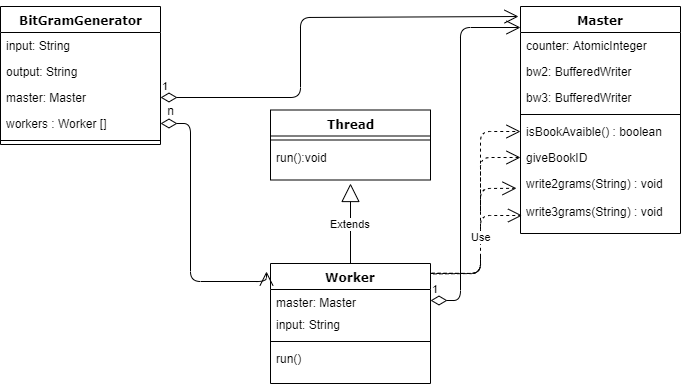
\includegraphics[width=\columnwidth]{template/latex/parallelUml.png}
\caption{UML of Parallel implementation.}
\label{fig:short}
\end{center}
\end{figure}
%-------------------------------------------------------------------------
\subsection{Hadoop implementation}

Hadoop version is implemented using a typical Map-Reduce's scheme.\\


\begin{figure}[H]
\begin{center}
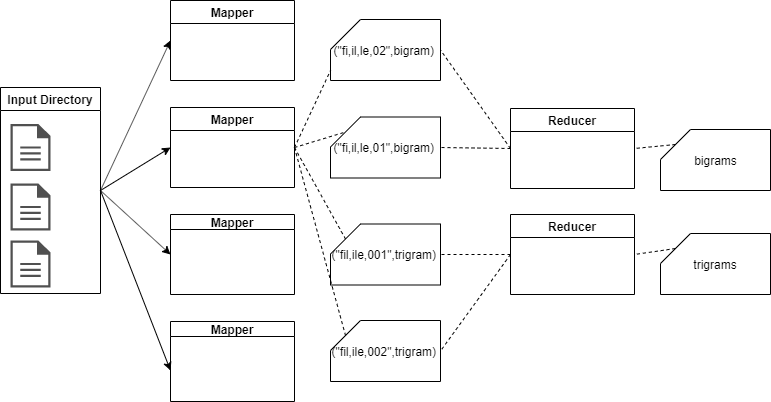
\includegraphics[width=\columnwidth]{template/latex/hadoop1.png}
\caption{Map-Reduce Scheme}
\label{fig:short}
\end{center}
\end{figure}
\vspace{2mm}
\begin{itemize}
    \item Mapper: mappers read and process books with the same logical of the others implementation.\\Output structure is context(key: Text, value: Text), where keys are the  codes ("bigram", "trigram").
    \item Reducer: reducers receive in input the same contexts type just described and write them in the correct output file, distinguishing them using the keys.
\end{itemize}

\section{Results}
\subsection{Test platform}

All the experiments are executed on a MSI GS65 with a i7-8750H 6 CORES 12 THREAD, 16 GB 2400 MHz DDR4 RAM and a M2 SSD SAMSUNG MZVLW256HEHP.

\subsubsection{Paralell implementation setup}

In the code we can choose the number of threads, which correspond to the number of workers, and the number of books processed each time a worker ask new books to process.\\
In the following test, this two variables are set respectively to 12 (6 cores,12 threads processors) and 1 due to different value of this parameter doesn't offer no significant improvement but without getting better result.

\subsubsection{AWS}

Emr cluster: 
\begin{itemize}
    \item m4.xlarge 1 master 4 slaves, Amazon Hadoop version's  2.8.5.
\end{itemize}
Storage:
\begin{itemize}
    \item S3 bucket.
\end{itemize}
\subsection{Tests}
\subsubsection{All version compared}

Below we report the result obtained from the first test and as expected we can see that hadoop is not suitable for our aim despite of the cluster used has significantly more resources than our test platform used for sequential/parallel's version.

\begin{figure}[H]
\begin{center}
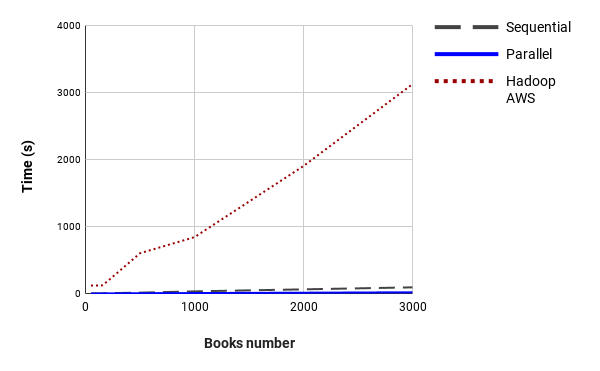
\includegraphics[width=\columnwidth]{template/latex/books.png}
\caption{All version compared respect to books number.}
\label{fig:short}
\end{center}
\end{figure}

\begin{table}[H]
\begin{center}
\begin{tabular}{|l|c|c|c|c|}
\hline
Books & Sequential & Parallel & Hadoop AWS\\
\hline\hline
50 & 1 [s] & 0 [s] & 120 [s]\\
100 & 2 [s] & 1 [s] & 120 [s]\\
150 & 2 [s] & 1 [s] & 120 [s]\\
200 & 4 [s] & 1 [s] & 180 [s]\\
500 & 13 [s] & 4 [s] & 600 [s]\\
1000 & 32 [s] & 7 [s] & 840 [s]\\
2000 & 62 [s] & 12 [s] & 1900 [s]\\
3000 & 92 [s] & 18 [s] & 3120 [s]\\
\hline
\end{tabular}
\end{center}
\caption{Runtimes of all version compared respect to books number.}
\end{table}

We also made a comparison between Hadoop on AWS and Hadoop on Standalone's mode only. The results confirm that, the management of  cluster nodes in distributed version, makes Hadoop  unsuitable for our use case, as expected.\\
Due to all these considerations for the next tests, we will delete Hadoop's result to emphasize differences between sequential and parallel implementation and to go deeper in the analysis.

\begin{figure}[H]
\begin{center}
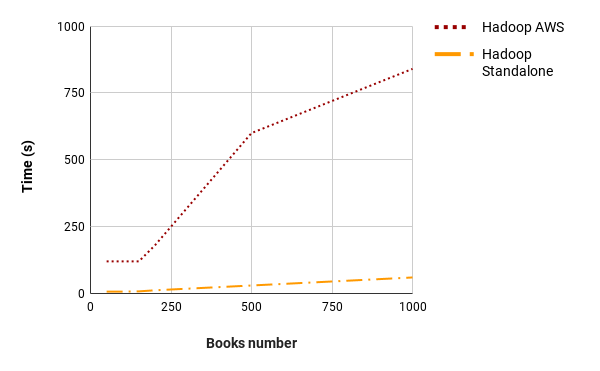
\includegraphics[width=\columnwidth]{template/latex/awsVsst.png}
\caption{Hadoop AWS Vs Hadoop Standalone respect to books number.}
\label{fig:short}
\end{center}
\end{figure}
\begin{table}[H]
\begin{center}
\begin{tabular}{|l|c|c|c|c|}
\hline
Books & Hadoop AWS & Hadoop Standalone\\
\hline\hline
50 & 120 [s] & 7 [s]\\
100 & 120 [s] & 7 [s]\\
150 & 120 [s] & 8 [s]\\
200 & 180 [s] & 12 [s]\\
500 & 600 [s] & 30 [s]\\
1000 & 840 [s] & 60 [s]\\
\hline
\end{tabular}
\end{center}
\caption{Runtimes of Hadoop AWS Vs Hadoop Standalone respect to books number.}
\end{table}
\newpage
\subsubsection{Parallel Vs sequential}

In figure 7, in which only the results of the parallel and sequential version are presented, allows us to appreciate better the advantage we can obtain by using parallel programming.

\begin{figure}[H]
\begin{center}
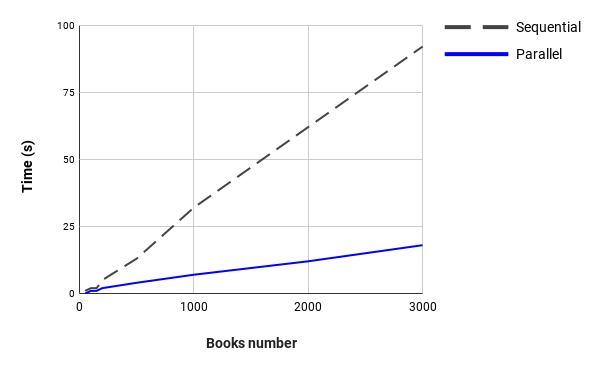
\includegraphics[width=\columnwidth]{template/latex/parVSseq.png}
\caption{Parallel Vs sequential respect to books number.}
\label{fig:short}
\end{center}
\end{figure}

\begin{table}[H]
\begin{center}
\begin{tabular}{|l|c|c|c|c|}
\hline
Books & Sequential & Parallel\\
\hline\hline
50 & 1 [s] & 0 [s]\\
100 & 2 [s] & 1 [s]\\
150 & 2 [s] & 1 [s]\\
200 & 5 [s] & 2 [s]\\
500 & 13 [s] & 4 [s]\\
1000 & 32 [s] & 7 [s]\\
2000 & 62 [s] & 13 [s]\\
3000 & 92 [s] & 18 [s]\\
\hline
\end{tabular}
\end{center}
\caption{Runtimes of parallel Vs sequential respect to books number.}
\end{table}

\begin{minipage}[H]{8.6cm}
Figure 8, with the speedup of parallel implementation respect to the sequential one, emphasizes the performance improvement .
\end{minipage}

\begin{figure}[H]
\begin{center}
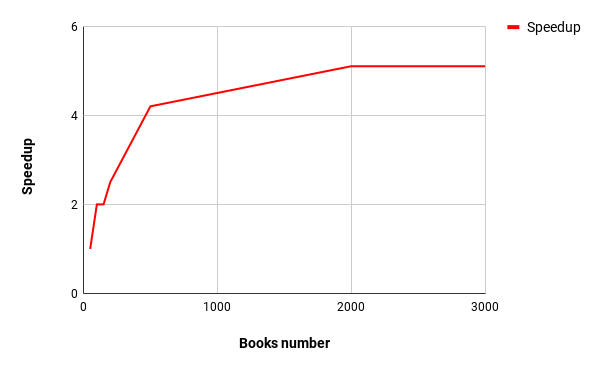
\includegraphics[width=\columnwidth]{template/latex/speedup.png}
\caption{Speedup parallel Vs sequential respect to books number.}
\label{fig:short}
\end{center}
\end{figure}

\begin{table}[H]
\begin{center}
\begin{tabular}{|l|c|c|c|c|}
\hline
Books & Speedup\\
\hline\hline
50 & 1x\\
100 & 2x\\
150 & 2x\\
200 & 2.5x\\
500 & 4.2x\\
1000 & 4.5x\\
2000 & 5.1x\\
3000 & 5.1x\\
\hline
\end{tabular}
\end{center}
\caption{Speedup parallel Vs sequential respect to books number.}
\end{table}

However, knowing that i/o intensive apps like this should benefit from a larger number of threads than the number of cores, we have test parallel implementation  with an increasing number of threads and these are the results.

\begin{figure}[H]
\begin{center}
\includegraphics[width=\columnwidth]{template/latex/parVsseqTh.png}
\centering
\caption{Parallel Vs sequential respect to number of threads.}
\label{fig:short}
\end{center}
\end{figure}

\begin{table}[H]
\begin{center}
\begin{tabular}{|l|c|c|c|c|}
\hline
Threads & Sequential & Parallel\\
\hline\hline
4 & 92 [s] & 26 [s]\\
6 & 92 [s] & 21 [s]\\
12 & 92 [s] & 17 [s]\\
24 & 92 [s] & 17 [s]\\
36 & 92 [s] & 17 [s]\\
48 & 92 [s] & 17 [s]\\
60 & 92 [s] & 17 [s]\\
\hline
\end{tabular}
\end{center}
\caption{Runtimes of parallel Vs sequential respect to number of threads.}
\end{table}

\begin{figure}[H]
\begin{center}
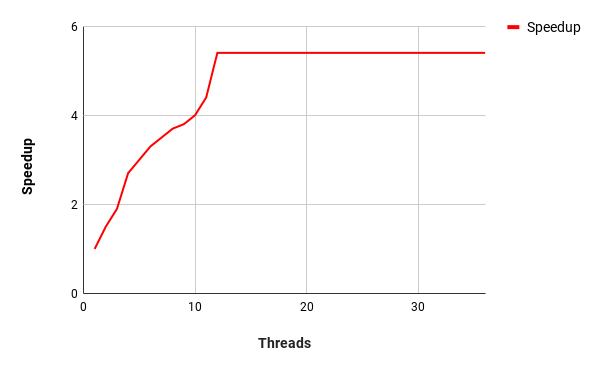
\includegraphics[width=\columnwidth]{template/latex/speedupTh.png}
\caption{Speedup parallel Vs sequential respect to number of thread.}
\label{fig:short}
\end{center}
\end{figure}

\begin{table}[H]
\begin{center}
\begin{tabular}{|l|c|c|c|c|}
\hline
Books & Speedup\\
\hline\hline
1 & 1x\\
2 & 1.5x\\
3 & 1.9x\\
4 & 2.7x\\
5 & 3x\\
6 & 3.3x\\
7 & 3.5x\\
8 & 3.7x\\
9 & 3.8x\\
10 & 4x\\
11 & 4.4x\\
12 & 5.4x\\
24 & 5.4x\\
36 & 5.4x\\
\hline
\end{tabular}
\end{center}
\caption{Speedup parallel Vs sequential respect to number of threads.}
\end{table}

We can see that the largest speedup obtained is with a number of threads equal to the number of cores and this was in contrast with what we saw during the course, we asked ourselves why and we thought it could be a limit given by the performance of the ssd, so we try to go deeper.
\subsubsection{Deeper Parallel Analysis}

\begin{figure}[H]
    \begin{center}
    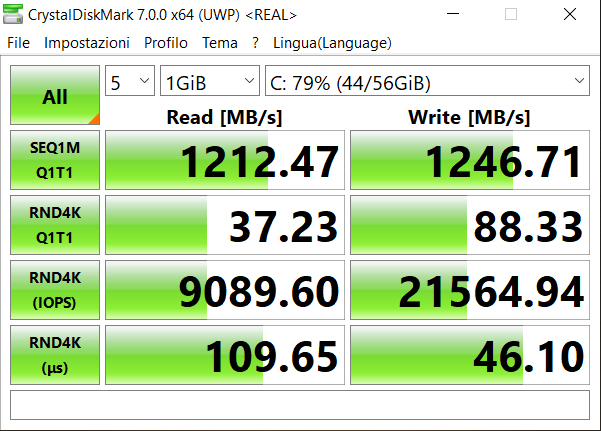
\includegraphics[width=\columnwidth]{template/latex/SSDbech.png}
    \caption{SSD benchmark.}
    \label{fig:my_label}
    \end{center}
\end{figure}


The ssd benchmark shows the lower limit to the program time given by the amount of data that pass through the program and the sequential read speed of the ssd. This test suggests that there is room for improvement.
However a test done with a program made by us that reads the books with the same scheme of the parallel program and rewrite them by duplicating the lines in the bigrams output and tripling those of the trigrams output only, to simulate the same data size, showing the same times  of our program. This confirms that the work added by the generation of bigrams and trigrams is almost irrelevant.


\begin{figure}[H]
\begin{center}
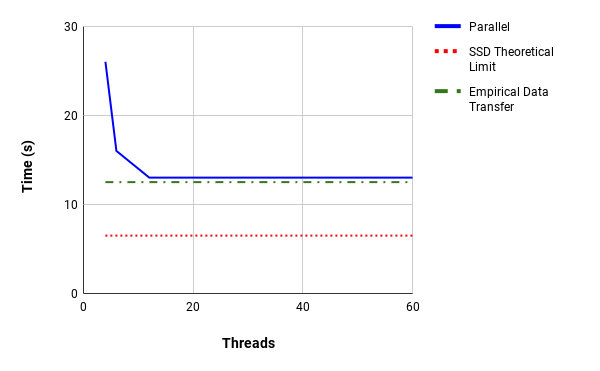
\includegraphics[width=\columnwidth]{template/latex/ssd.png}
\end{center}
\end{figure}

%\begin{table}[ht]
%\begin{center}
%\begin{tabular}{|l|c|c|c|c|}
%\hline
%Threads & Par. & SSD Theor. Limit & Emp. Data Transfer \\
%\hline\hline
%4 & 26 [s] & 6.5 [s] & 12.5 [s]\\
%6 & 16 [s] & 6.5 [s] & 12.5 [s]\\
%12 & 13 [s] & 6.5 [s] & 12.5 [s]\\
%24 & 13 [s] & 6.5 [s] & 12.5 [s]\\
%36 & 13 [s] & 6.5 [s] & 12.5 [s]\\
%48 & 13 [s] & 6.5 [s] & 12.5 [s]\\
%60 & 13 [s] & 6.5 [s] & 12.5 [s]\\
%
%\hline
%\end{tabular}
%\end{center}
%\caption{Execution Time.}
%\end{table}
Therefore probably the time difference is due to the fact that the books are many small files that must be opened and read in succession.
We think this does not lead to take advantage of the SSD's great sequential read speed.

\section{Conclusions}
After exploring different Java approaches in the case of bigrams and trigrams generation we can summarize that the parallel approach, as expected, certainly gives great advantages.
However, in the classic case of Hadoop usage, it is performed local computations over huge amounts of input data while returning relatively small result set, which makes our case  not  suitable to be implemented with Hadoop.\\
If instead we had to create a program for n-grams counting rather than writing them only, probably we would have been able to see the potential of this distributed technology.



{\small
\bibliographystyle{ieee}
\bibliography{egbib}
aws.amazon.com.
}



\end{document}
